% Homework through lecture6. Compile with LuaLaTeX + BibTeX.
\documentclass{article}
\PassOptionsToPackage{numbers,sort,compress}{natbib}
\usepackage[preprint]{neurips_2025}
\usepackage{fontspec}
\setmainfont{Liberation Serif}
\setsansfont{DejaVu Sans}
\setmonofont{DejaVu Sans Mono}[Scale=MatchLowercase]
\usepackage{polyglossia}
\setdefaultlanguage{russian}
\setotherlanguage{english}
\usepackage{amsmath,amssymb,booktabs,graphicx,hyperref}
\setlength{\emergencystretch}{3em}
\hypersetup{colorlinks=true,linkcolor=blue,citecolor=blue,urlcolor=blue}
\makeatletter
\renewcommand{\@noticestring}{Материалы ДЗ до шестой лекции. Курс «Моя первая научная статья», осень 2026.}
\makeatother
\title{Выбор политики маршрутизации в двухмодельных каскадах:\\
влияние данных, структуры ошибок и вычислительного бюджета}
\author{Anastasia Shlopak\\Научный руководитель: Archil Maysuradze, PhD}
\begin{document}
\maketitle
\begin{abstract}
Каскадные системы позволяют адаптивно распределять вычислительные ресурсы, передавая часть запросов от дешёвого предиктора более дорогому. Эффективность такой системы зависит от способности маршрутизатора оценить ожидаемое изменение качества ответа: дорогая модель может как исправить ошибку, так и заменить правильный ответ неправильным. Существующие маршрутизаторы используют различные обучающие цели и параметризации, однако для выбора того или иного подхода для новой задачи важно учитывать доступные данные, структуру ошибок моделей и ограничения эксплуатации. Цель исследования заключается в выявлении условий, при которых различные способы обучения маршрутизатора будут обеспечивать наилучшее соотношение качества и вычислительных затрат. Основная задача - разработать систему рекомендаций по выбору маршрутизатора на основе характеристик данных и используемых моделей. В работе будет рассматривается каскад из двух фиксированных классификаторов и маршрутизатора, получающего на вход признаки объекта и результат дешёвой модели. Для сравнения будут выбраны такие политики маршрутизации как прямая регрессия прироста качества, разность оценок правильности моделей, оценивание вероятностей исправления и ухудшения качества ответа, неуверенность только дешевой модели, сложность признаков входного объекта. Переносимость сформированных рекомендаций планируется проверить на новых наборах данных и парах классификаторов, не использованных при выявлении закономерностей и выборе параметров методов. Итогом работы должны стать экспериментально обоснованные правила выбора способа обучения маршрутизатора, позволяющие определить, когда дополнительная сложность оправданна, а когда сопоставимое качество достигается более простым решением.

\end{abstract}
\noindent\textbf{Ключевые слова:} каскад классификаторов, маршрутизация,
ожидаемая полезность, парная разметка, совместные ошибки, выбор метода обучения.

\section{Введение}
Каскадная обработка позволяет выделять дополнительное вычисление запросам,
на которых оно полезно. Первая модель отвечает всегда, после чего
маршрутизатор сохраняет её ответ либо передаёт запрос второму эксперту.
Поскольку второй эксперт тоже ошибается, более высокая средняя accuracy
не гарантирует полезность каждого перехода. Исследование посвящено выбору
способа обучения такого маршрутизатора для заданных данных, пары моделей
и бюджета.

Сравнительная полезность эскалации уже формализована в литературе.
\citet{jitkrittum2023confidence} рассматривают разность вероятностей
правильности и прямую регрессию signed gain, а также условия достаточности
confidence-правила. Post-hoc обучение связано с передачей решения
ошибающемуся эксперту \citep{narasimhan2022posthoc}; для языковых моделей
изучены token-level признаки \citep{gupta2024cascades} и выбор продолжения
по ожидаемой полезности \citep{aggarwal2024automix}. Работа опирается
на эти результаты, а не заявляет новую целевую функцию.

Остаётся практический вопрос, как выбирать между оценивателями при
конечном объёме парной разметки. Разные источники/составы обучения
по-разному влияют на роутеры \citep{ong2025routellm,niu2026routing}.
В uplift modeling уже показаны искажение оценки эффекта после
пересэмплирования и роль поддержки редких событий \citep{nyberg2023exploring}.
Поэтому требуется объяснить конкретные режимы, а не ограничиваться
утверждением, что результаты зависят от данных.

Предлагается фиксировать экспертов и доступные признаки, менять объём
и состав именно обучения роутера и сравнивать методы при одной квоте
эскалаций. Дополнительно к accuracy рассматриваются таблицы решений:
исправленные ошибки, вредные замены, упущенные спасения и предотвращённый
вред. Цель --- установить условия предпочтительности способов обучения
и затем проверить рекомендации на новых задачах и парах моделей.

Первый эксперимент использует BANKING77 и предвычисленные прогнозы
независимо обученных классификаторов. В этих материалах оформлены
постановка и базовое сравнение трёх обучаемых правил с confidence,
кривая ошибки и описательный пример профилей решений. Профили пока
не прошли отдельную статистическую проверку; переносимые рекомендации
ещё не получены. Это текущий этап работы, а не завершённая статья.

\section{Постановка задачи}
Даны запросы и эталоны $(x,y)\sim P$, два фиксированных классификатора
$M_w,M_s$ и парная обучающая разметка их правильности:
$W=\mathbf1\{M_w(x)\text{ правилен}\}$,
$S=\mathbf1\{M_s(x)\text{ правилен}\}$, $D=S-W$.
Роутер использует $z=\phi(x,M_w(x))$, доступные до вызова $M_s$ признаки;
эталон и текущий ответ второй модели при решении неизвестны.
После эскалации второй ответ заменяет первый. Искомая полезность:
\begin{equation}\label{eq:gain}
\begin{aligned}
g(z)&=\mathbb E[D\mid z]\\
&=P(W=0,S=1\mid z)-P(W=1,S=0\mid z).
\end{aligned}
\end{equation}
Спасению соответствует $D=1$, вреду $D=-1$, одинаковой правильности
обоих ответов $D=0$. Для решения $r(z)\in\{0,1\}$ внешний критерий:
\begin{equation}\label{eq:quality}
 Q(r)=\mathbb E[W+r(z)D],\qquad
 \mathbb E[c_w+c_{\phi,r}+r(z)c_s]\le B.
\end{equation}
Первый вызов уже оплачен, добавочная стоимость --- $c_s$.
В базовом опыте фиксируется ровно $k=\lfloor bN\rfloor$ вторых вызовов
на batch из $N$ запросов: top-$k$ по оценке gain с общим разрешением ties.
Это квота, а не проверенный online-порог или денежный бюджет.

Для разбора решения относительно противоположного действия определим
$Z_r=(2r-1)D$ и таблицу $T_{v,a}=\sum_i\mathbf1\{Z_{r,i}=v,r_i=a\}$.
В колонке эскалации $+1$ означает спасение, $-1$ --- вред; без эскалации
$+1$ означает предотвращённый вред, $-1$ --- упущенное спасение.
Нейтральный исход включает как два правильных, так и два ошибочных ответа.
При числе спасений $R$ и вредных замен $H$ эмпирический прирост accuracy
равен $(R-H)/N$: таблица раскрывает компоненты агрегированной метрики.

Expert-train, router-fit, policy-dev и test разделяются. Scaler и параметры
роутера обучаются только на выбранном router-fit; регуляризация выбирается
на dev, test используется для отчёта. В базовом direct-варианте ищется
функция $f_\theta$ линейного семейства с внутренним MSE-критерием:
\begin{equation}\label{eq:argmin}
\widehat\theta_\lambda\in\arg\min_\theta
\left\{\frac1n\sum_{i=1}^{n}(D_i-f_\theta(z_i))^2+
\lambda\|\theta_{\mathrm{coef}}\|_2^2\right\}.
\end{equation}
Intercept не штрафуется. Для вероятностных голов используется log-loss.
На уровне всего исследования требуется выбирать способ обучения по
разрешённым характеристикам train/dev с малой потерей относительно
лучшего кандидата на новых задачах; этот выбор не делается по test.

\section{Базовый вычислительный эксперимент}
\textbf{Цель} --- проверить реализацию и сравнить ошибку и профили решений
роутеров при фиксированных экспертах/признаках и одинаковой квоте.
Используется BANKING77: 77 банковских намерений, источник
\citet{review17}, PolyAI revision
\texttt{57ec275d8078af65b7731c2a98be812d844a6d6b}, CC BY 4.0.
После удаления четырёх train-повторов остаётся 9\,999 примеров:
expert-train 5\,999, calibration 1\,000, router-fit 2\,000, policy-dev 1\,000.
Official test 3\,080 сохранён; чувствительность без известных текстовых
пересечений/повтора оценивается на 3\,072 строках. Между train-частями
пересечений нет. Seeds и SHA зафиксированы в manifest.

Две пары: TF--IDF+LR (accuracy 86.56\%) с BERT-tiny (84.71\%) либо
frozen MiniLM+LR (92.31\%). Все эксперты фиксированы до обучения роутера;
дорогой эксперт не обязан быть точнее. Сравниваются confidence,
logistic weak-error, ridge direct и две logistic rescue/harm-головы.
Восемь признаков: max probability, top-two margin, энтропия, сумма
квадратов вероятностей, вторая/третья вероятности и log1p длины запроса
в символах/словах. Правильность экспертов не является входным признаком.

Выполнены fit 200/500/1\,000, dev=fit/2, 10 подвыборок,
квоты 10/20/40\%. Одинаковые fit/dev строки и tie keys используются всеми
методами внутри условия. L2-grid: $\{0.001,0.01,0.1,1\}$;
критерий настройки --- MSE наблюдаемого $D$ на естественном dev.
Количество доступных пар включает настройку. Линейные/logistic правила
малые, но не строго capacity-matched.

\begin{table}[htbp]\centering
\caption{TF--IDF $\to$ frozen MiniLM, natural fit 1\,000/dev 500,
20\% эскалаций. Средние и SD по 10 подвыборкам; SD не является CI
из независимых задач.}\label{tab:base}
\begin{tabular}{lrr}
\toprule
Способ & Accuracy, \% & SD, п.п. \\
\midrule
confidence & 90{,}68 & 0{,}00 \\
weak\_error & 91{,}27 & 0{,}07 \\
direct & 91{,}48 & 0{,}23 \\
events & 91{,}53 & 0{,}17 \\
\bottomrule
\end{tabular}

\end{table}
\begin{figure}[htbp]\centering
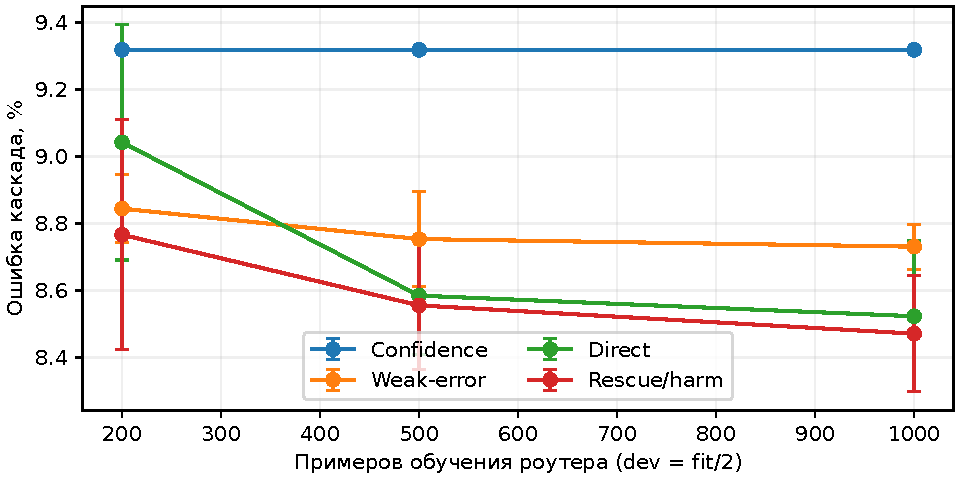
\includegraphics[width=.82\linewidth]{figures/error_curve.pdf}
\caption{Ошибка каскада при изменении fit и dev=fit/2,
TF--IDF $\to$ frozen MiniLM, 20\% эскалаций. Полосы --- SD по 10
подвыборкам. Кривая построена после выполненного опыта; она не
выдаётся за доруновый карандашный эскиз.}\label{fig:error}
\end{figure}

Базовый результат приведён в таблице~\ref{tab:base} и на
рисунке~\ref{fig:error}. При увеличении доступного обучения ошибка
части правил снижается; различия средних не объявляются значимыми
на основании одной кривой. Пример на рисунке~\ref{fig:profiles}
показывает обмен между исправлениями и вредом: confidence исправляет
123 ответа и портит 102, Events --- в среднем 85.2 и 51.1.
Вмешательств с изменением правильности меньше в обоих направлениях.
Это описательный пример, выбранный после просмотра пилота; отдельная
проверка значимости компонент пока не выполнена. Более широкий
разбор accuracy с общей статистической поправкой не установил
убедительного преимущества способов маршрутизации.

\begin{figure}[htbp]\centering
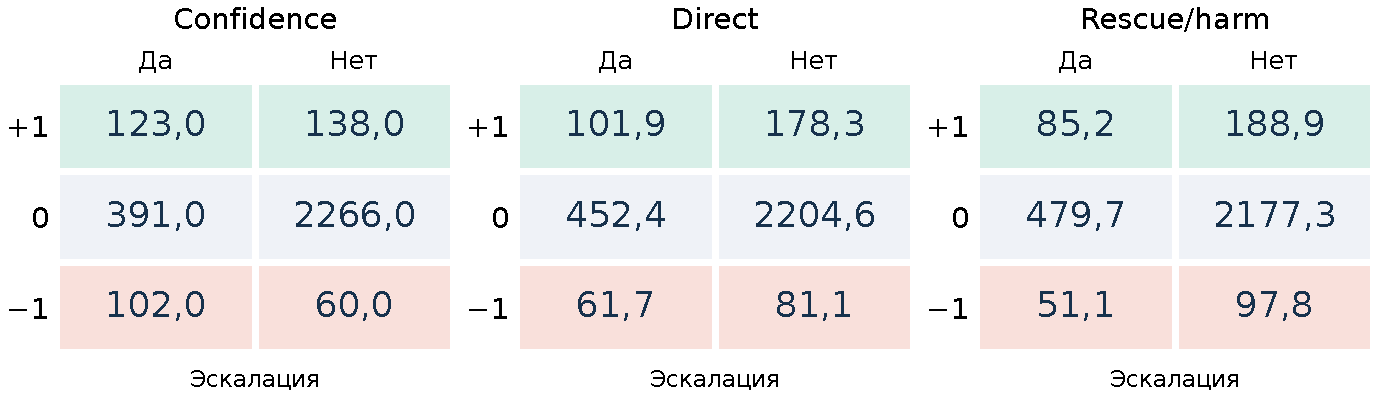
\includegraphics[width=\linewidth]{figures/decision_profiles.pdf}
\caption{Главный рисунок: TF--IDF $\to$ BERT-tiny, fit 1\,000/dev 500,
20\% вызовов (616 из 3\,080), средние counts по 10 обучениям.
Строки --- $Z_r$ относительно противоположного действия; колонки ---
эскалация да/нет. Профили различаются описательно, не доказано
статистическое превосходство одного правила.}\label{fig:profiles}
\end{figure}

\paragraph{Воспроизведение.}
\url{https://github.com/Nastik05/Cost-sensitive-routing}:
\texttt{python3 code/run.py} заново обучает роутеры по компактному кэшу,
проверяет все 1\,440 строк метрик против исходного прогона и строит
рисунки/таблицу TeX. Это не переобучение экспертов и не новый test.
Реализация вычислений и рисунков разделена. Числа статьи получаются
из результатов автоматически; source revision и параметры экспертов
сохранены в \texttt{code/data/manifest.json}.

\paragraph{Следующий этап.}
Проверить роль состава обучения и отдельно скорректировать смещение
отбора, исследовать профили решений и подтвердить рекомендации
на новых задачах. Малые различия accuracy и отсутствие значимости
не означают эквивалентность. Сама таблица спасений/вреда не заявляется
новым методом; исследовательская цель --- условия выбора обучения.

\bibliographystyle{unsrtnat}
\bibliography{references}
\end{document}
